\ylDisplay{Takistid} % Ülesande nimi
{Tundmatu autor} % Autor
{lõppvoor} % Voor
{2017} % Aasta
{P 8} % Ülesande nr.
{3} % Raskustase
{
% Teema: Elektriõpetus

\ifStatement
Leidke takistus punktide $A$ ja $B$ vahel. Iga takisti takistus on $R$.
\begin{center}
	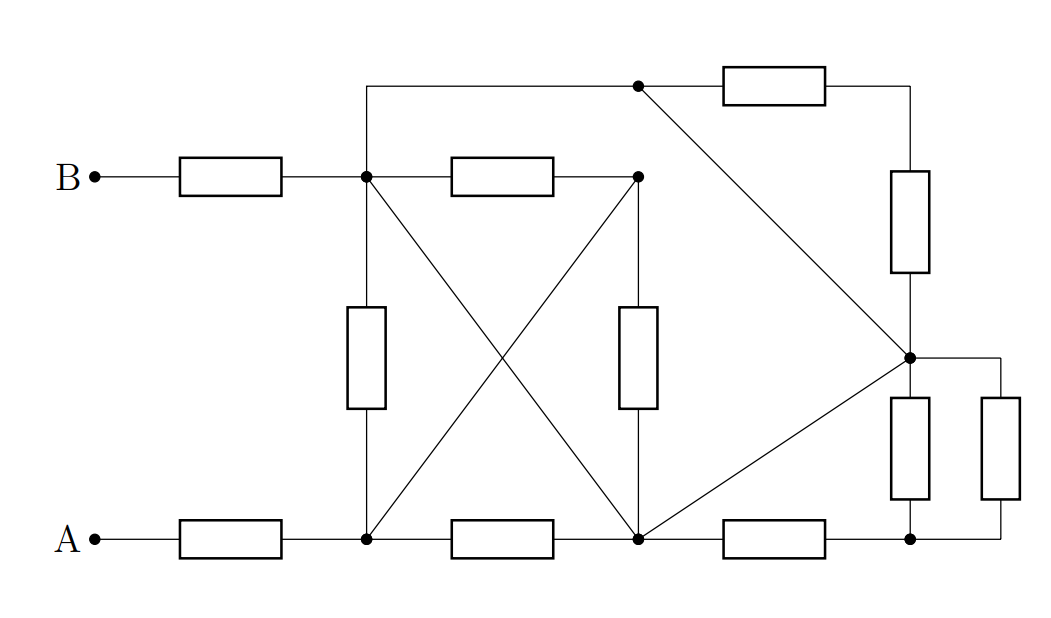
\includegraphics[width=0.5\linewidth]{2017-v3p-08-yl.png}
\end{center}
\fi

\ifHint
Ülesande lahendamiseks on mõistlik esialgset skeemi lihtsustada, hinnates, millised vooluringi osad võiks skeemilt välja jätta ning millised saaks lihtsamateks osadeks taandada.
\fi

\ifSolution
Tähistame skeemil olevad punktid järgnevalt:
\begin{center}
	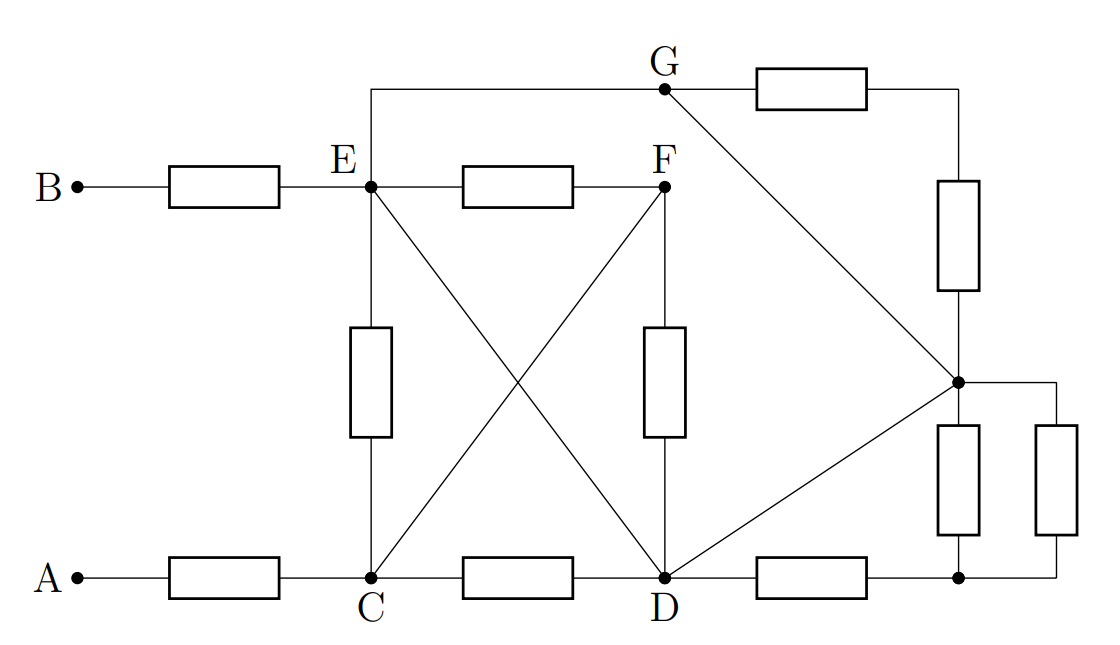
\includegraphics[width=0.5\linewidth]{2017-v3p-08-lah1.png}
\end{center}

Punktid $E$ ja $D$ on ühendatud otse juhtmega ja ka läbi takistite, mis asuvad punktidest $D$ ja $G$ paremal. Kui kaks punkti on juhtmega ühendatud, siis on pinge nendes punktides sama. Seega on pinge punktidest $D$ ja $G$ paremal asuvatel takistitel null ja vool neid ei läbi. Võime need takistid ära jätta ja saame järgneva skeemi:
\begin{center}
	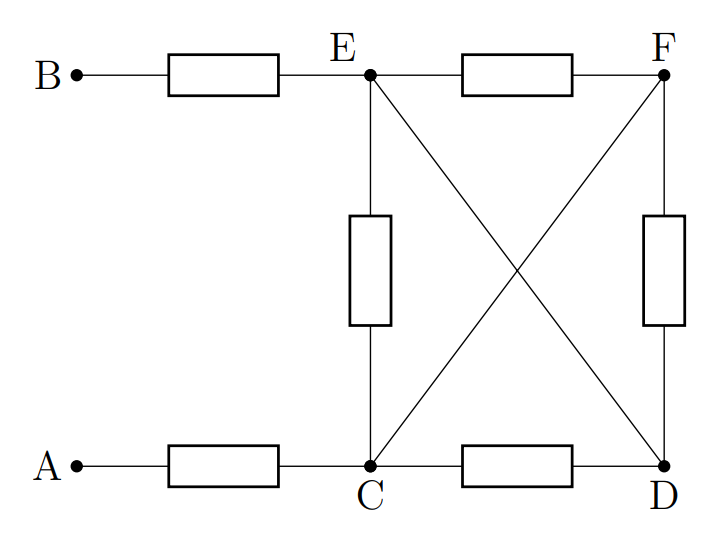
\includegraphics[width=0.5\linewidth]{2017-v3p-08-lah2.png}
\end{center}
Mõtleme, kuidas saab vool minna punktist $C$ punkti $4$. Selleks on neli võimalust, liikudes otse punktist $C$ punkti $E$ või läbides punkte $CDE$, $CFE$ või $CFDE$. Iga kord liigub vool läbi ühe takisti. Sisuliselt on tegemist nelja takisti paralleelse ühendusega. Seega on punktide $C$ ja $E$ vaheline takistus $\frac{R}{4}$ ja saame skeemi:
\begin{center}
	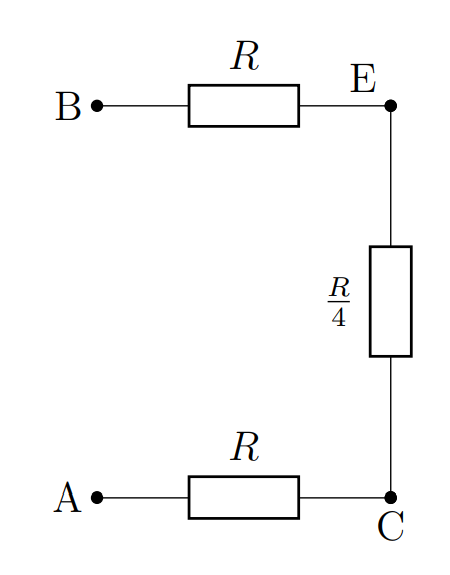
\includegraphics[width=0.5\linewidth]{2017-v3p-08-lah3.png}
\end{center}

Selles skeemis on kolm takistit jadamisi ühendatud. Punktide $A$ ja $B$ vahelise kogutakistuse leidmiseks tuleb need kokku liita, mis annab $R + R + \frac{R}{4}= \frac{9}{4}$  $R$.
\fi
}